\documentclass[twocolumn,letterpaper]{article}

\usepackage{url}
\usepackage{graphicx}
\usepackage{caption}
\usepackage{subcaption}
\usepackage[margin=1in]{geometry}
\usepackage{gensymb}
\usepackage{lipsum}

%opening
\title{NeuroEvolution of Augmenting Topologies}
\author{Nathan Zabriskie}

\begin{document}

\maketitle

\section{Introduction} \label{sec:intro} 
Genetic algorithms learn by heuristically sampling possible solutions to some problem, assigning a fitness
score to each solution based on its performance, and then combining and tweaking the most 
``fit'' solutions to create more samples for the next step of the simulation. Traditionally, 
genetic algorithms would operate on a fixed network topology specified by the user, with each 
genome representing some possible weights for connections within the network. Although
researchers made some early attempts to develop genetic algorithms that evolved topologies along with 
weights (called Topology and Weight Evolving Artificial Neural Networks or TWEANNs), 
these algorithms often suffered from a number of problems including information loss due to competing 
conventions and overly penalizing new, larger topologies. 

In \textit{Evolving Neural Networks through Augmenting Topologies} \cite{neat_paper} Stanley and 
Miikkulainen present their algorithm NeuroEvolution of Augmenting Topologies (NEAT) which addresses some of
these problems. This paper examines the contributions of NEAT and evaluates its performance on a number
of tasks.

\section{NEAT Overview} \label{sec:overview}
As mentioned above, early TWEANN models often suffered from information loss during the crossover phase
at the end of each generation due to what Stanley and Miikulainen term the competing conventions problem.
When two genomes contain hidden nodes that encode the same information, if their hidden nodes are stored 
in different orders their offspring will invariably lose the capabilities of at least one of the 
hidden nodes as shown in figure \ref{fig:crossover_loss}. 

NEAT addresses this problem by assigning each connection within the network an innovation number based on
when the connection first appears. Each time a connection is added during the offspring creation phase at the end of a generation it is compared with other connections that have appeared in the same generation. 
If a matching connection is found then the connection is assigned the same innovation number as the earlier
connection, otherwise it is given a new, unique number. In future generations when performing crossover,
connections are aligned according to their innovation numbers which helps prevent loss due to competing
conventions. 

\begin{figure}[h]
	\centering
	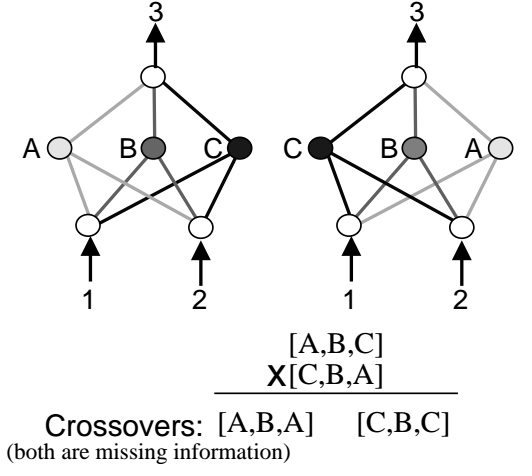
\includegraphics[width=0.3\textwidth]{images/crossover.png}
	\caption{Information loss due to crossover.}
	\label{fig:crossover_loss}
\end{figure} 

Tracking connections in this way also helps solve another problem in TWEANN's, the penalizing of new
developments. In order to encourage the development of simple networks many TWEANN algorithms add a penalty
term to fitness calculations based on the number of nodes in a network. Although this will in theory keep
networks small, it can have some unintended side effects. Often when a new node is added to a network
it takes some number of generations before the node develops any useful function and contributes to the 
genome' fitness. If a genome with a new node is overly penalized just for having an extra node it might be
eliminated from the population before it has a chance to develop thus preventing what could potentially be a
useful new development.

NEAT solves this problem by organizing genomes into species based on how similar each genome is to each other.
Although NEAT is not the first algorithm to speciate genomes, the tracking of innovation numbers makes
calculating the distance between genomes trivial. Again connection genes within each genome are simply
aligned according to their innovation numbers and the number of differing genes are counted. Then the distance
$\delta$ between the two genomes is calculated by
\begin{equation}
\delta = \frac{c_1E}{N}\ + \frac{c_2D}{N}\ + c_3\overline{W}
\end{equation}
where $E$ is the number of excess genes (genes in one genome that have higher IDs than the maximum
ID in the other genome), $D$ is the number of disjoint genes, $\overline{W}$ is the average weight
difference between matching genes, and $c_1$, $c_2$, and $c_3$ are user-defined constants. Genomes with 
$\delta$ smaller than some value are put into the same species and compete only within that species. If a
species does not improve its fitness for a number of generations then it is eliminated. By protecting new
innovations in this way, new developments are given time to develop but are eventually trimmed out if they 
fail to produce positive results.

\begin{figure}[b]
	\centering
	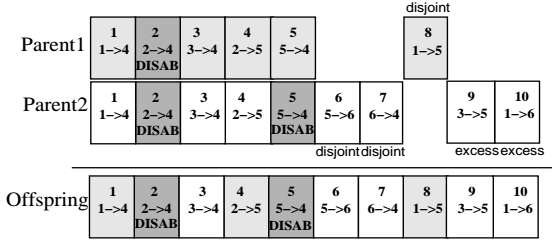
\includegraphics[width=0.5\textwidth]{images/speciation.png}
	\caption{Aligning genomes by innovation number simplifies the counting of differing genes.}
	\label{fig:speciation}
\end{figure}
  
\section{Experiments} \label{sec:experiments}
Although genetic algorithms can be used to do supervised learning, often their performance lags behind
more mathematically rigorous methods such as simple back-propagation. After ensuring that my implementation of NEAT worked correctly, I tested my model on several classic datasets such as the iris and diabetes datasets but I was very unimpressed by the
results. Although the final accuracies on these problems was comparable to standard neural networks, NEAT was 
much slower to train and very sensitive to overfit. I eventually moved on to reinforcement learning tasks
because as detailed in \cite{whitley} genetic algorithms excel in situations where gradients are difficult to
calculate and standard gradient-descent algorithms break down. As the reinforcement learning tasks better
showcase the strengths of this model this section will primarily deal with those experiments. NOTE: In all
network diagrams green nodes are inputs, blue nodes are outputs, black edges represent forward connections,
red edges represent recurrent connections, and dashed lines represent disabled connections that have no
effect.

\subsection{XOR Verification} \label{sec:xor}
I used the XOR task to ensure that my NEAT implementation worked properly as Stanley and 
Miikkulainen explicitly mention it in their paper as a good test problem. For this experiment I 
initialized a population of 150 genomes to each have 2 input nodes and 1 output node. Each genome received
a fitness calculated by the formula 
\begin{equation}
fitness = (4-\sum_{n} \left|t_n-z_n\right|)^2 
\end{equation}
where $t_n$ is the desired output for input \textit{n} and $z_n$ is the actual output for each of the 4
possible inputs. After I discovered and fixed several bugs the system performed quite well on this task. 
In no run did it fail to find a solution and over 10 runs the final network had an average of 2.6 hidden
nodes where 1 is optimal. Although it did not find the optimal solution in every run it did develop a 
network with 1 hidden node in $\approx20\%$ of runs.

\begin{figure}[h!]
	\centering
	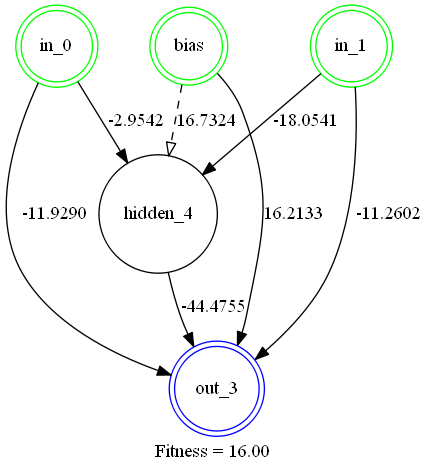
\includegraphics[width=0.2\textwidth]{images/xor_end.png}
	\caption{An example XOR solution}
	\label{fig:xor}
\end{figure}

\subsection{Flappy Bird} \label{sec:flappy}
After I was satisfied that my system was working correctly, I created a reinforcement learning environment by hooking my NEAT implementation up to the Bizhawk
Nintendo Entertainment System emulator and had it learn to play the game Flappy Bird. In Flappy Bird the player is tasked with guiding a bird through a series of vertical gaps by having the bird
flap its wings to gain height. This sounds simple enough but it turns out to be a very difficult game for a
human player due to the unforgiving collision detection and narrow gaps.

\begin{figure}[t]
	\centering
	\begin{subfigure}[b]{0.45\textwidth}
		
\includegraphics[width=\textwidth]{images/flappy.png}
		\caption{A frame from the Flappy Bird simulation}
	\end{subfigure}
	~
	\begin{subfigure}[b]{0.3\textwidth}
		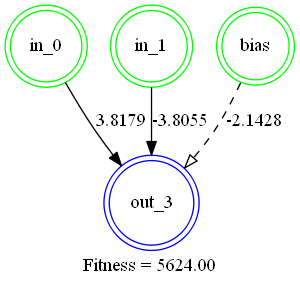
\includegraphics[width=\textwidth]{images/flappy_network.png}
		\caption{An example solution network}
		\label{fig:flappy_network}
	\end{subfigure}
	\caption{Flappy Bird reinforcement learning task}
	\label{fig:flappy}
\end{figure}

Unfortunately, Bizhawk
can only interact with Lua scripts whereas I implemented NEAT in Python. To communicate between these
platforms I created a server that runs NEAT in a Python environment and receives commands over a socket
connection. The Lua client simply sends commands to the server to end a generation, get a genome's output,
or assign a fitness score to a genome. Although this adds some undesired overhead, this setup was more than fast enough to handle all the commands necessary to run the emulator at full speed and quickly iterate
through generations.

 In order to get any meaningful 
information out of the emulator it is necessary to read values out of the game's RAM which I had not had 
previous experience with. Luckily I was able to determine how to get the current height of the bird and
the height of the next upcoming gap so these two values served as the inputs to the system. Each genome
had to take these two inputs and then return whether the bird should flap its wings or stay idle. Genomes
received a fitness based on how many frames they survived plus a bonus for each gap they successfully 
navigated.

Using only these two inputs NEAT created an agent that could play the game indefinitely in an average of
11.3 generations. As shown in figure \ref{fig:flappy_network} the networks that evolved were not complicated
but they performed very well. While watching the agents play the game I noticed that a large number of the 
agents in early generations would press the flap button at every possible opportunity, quickly flying off the top of the
screen. This prevents them from crashing into the ground immediately but also prevents them from ever clearing
one of the vertical gaps. To discourage this behavior I eventually added a penalty term to the fitness
calculation for every flap taken. This penalty helped focus the efforts of the genomes and decreased the
average number of generations required to 4.6.  
 
\subsection{Pole Balancing}  \label{sec:pole}
Since Flappy Bird ended up being a little on the easy side, I moved on to what I hoped would be a more
difficult reinforcement learning task. As described in \cite{cartpole}, the pole balancing problem is a classic control task
in which systems must balance an inverted pendulum on a cart by pushing the cart left or right. The original
formulation of the problem provides the agent with 4 observations at each time step: the position of the
cart, the velocity of the cart, the angle of the pole, and the velocity of the tip of the pole. 

At each step 
of the simulation the agent is provided with the 4 observations and must return its chosen action, to push
the cart left or to push the cart right. In the Python OpenAI Gym \cite{gym} the simulation ends when the
pole angle is $> 20.2^{\circ}$ from vertical or the cart is $> 2.4$ units from the center of the track. For each
frame the agent survives, its fitness increases by one point. The problem is considered solved when an agent
receives $> 475$ fitness averaged over 100 runs. 

\begin{figure}[h]
	\centering
	\begin{subfigure}[b]{0.3\textwidth}
		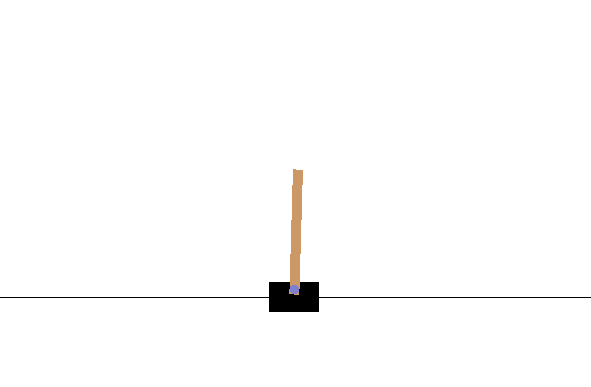
\includegraphics[width=\textwidth]{images/pole_balance.png}
		\caption{Example frame of the cart pole simulation.}
	\end{subfigure}
	~
	\begin{subfigure}[b]{0.3\textwidth}
		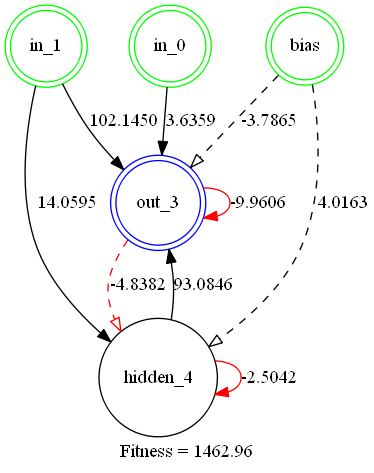
\includegraphics[width=\textwidth]{images/cart_pole_final.png}
		\caption{An example solution.}
		\label{fig:cart_solution}
	\end{subfigure}
	\caption{The pole balancing problem with withheld velocity}
	\label{fig:cartpole}
\end{figure}

Using all 4 observations, NEAT solved the problem using the initial population in $\approx80\%$ of runs, meaning
that the system never had to change a single genome in order to achieve the required fitness. This is not
particularly interesting so I decided to increase the challenge of the problem by only providing each network
with the positions of the cart and pole, withholding the velocity. Under these conditions the system must
evolve recurrent connections in addition to the normal forward connections in order to recover the missing
information. Even with the missing information NEAT handled the problem very nicely. Over 10 runs it solved
the problem in an average of 109 generations. Figure \ref{fig:cart_solution} shows a particularly
appealing solution with only one hidden node. Although it's difficult to determine exactly what each 
connection represents, the two active recurrent connections indicate that the system retains some history
of previous positions in order to reconstruct the velocity.  

\section{Modifications} \label{sec:mods}
In order to better understand the reasoning behind some design decisions in the original NEAT algorithm I made
several modifications to the base system.

\subsection{Speciation} \label{sec:speciation}
While experimenting with the NEAT algorithm I was often frustrated by how sensitive it was to the changes
in its hyper parameters. Often it would take many runs to find parameters that allowed the system to find a
solution and any small perturbations to these parameters would drastically influence run times. One 
particularly sensitive parameter was the distance threshold for $\delta$ that determines whether two genomes
are in the same species or not. If this threshold was too low then the number of species would explode. If
it was too high then there would only be one species and the system would not have enough diversity.

\begin{figure}[h]
	\centering
	\begin{subfigure}[b]{0.3\textwidth}
		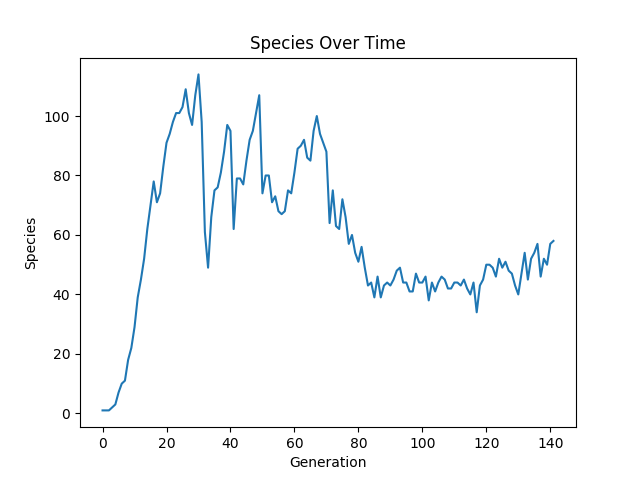
\includegraphics[width=\textwidth]{images/no_adjust.png}
		\caption{Species over time with no dynamic threshold}
		\label{fig:no_adjust}
	\end{subfigure}
	~
	\begin{subfigure}[b]{0.3\textwidth}
		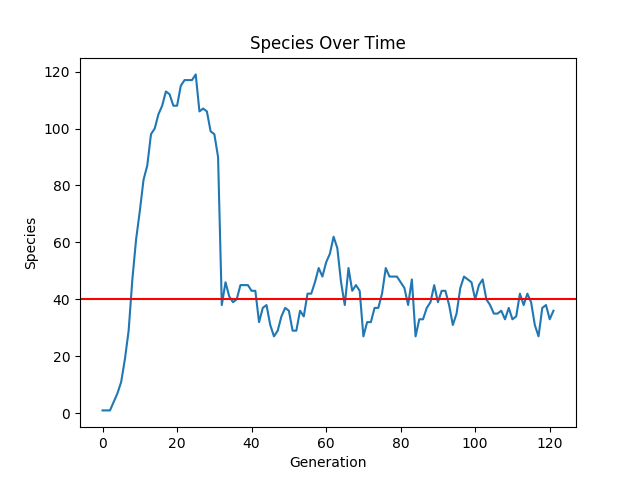
\includegraphics[width=\textwidth]{images/with_adjust.png}
		\caption{Species over time with dynamic threshold. The target number of species is marked with a red line}
		\label{fig:with_adjust}
	\end{subfigure}
	\caption{Effects of dynamic $\delta$ threshold}
	\label{fig:speciation_adjustment}
\end{figure}

While searching for how other people dealt with this problem I came across \cite{neat_web}, a website created
by one of the original paper authors, that has some helpful information about how to improve stability in
NEAT. One item suggested making the $\delta$ threshold dynamic in order to maintain a target number of
species. Making this addition proved very useful. With this change I simply set the threshold to 
a reasonable value and let the system run. Figure \ref{fig:speciation_adjustment} shows the effects of
making this threshold dynamic. It is worth mentioning that although figure \ref{fig:no_adjust} and 
\ref{fig:with_adjust} look similar, this is mostly due to the fact that figure \ref{fig:no_adjust} was
generated only after testing many threshold values to find one that allows the system to find a solution
whereas \ref{fig:with_adjust} was generated in one shot.
 
\subsection{Innovation Tracking} \label{sec:innovations}
During my initial reading of \cite{neat_paper} I found it odd that innovation numbers were only shared among
connections created during the current generation instead of among all connections in every network. It seemed to me that by always connections that connected the same nodes the same ID you could decrease the
number of connections present in the final solution. To test this hypothesis I ran the pole balancing problem
5 times with the default ID sharing strategy and 5 times with the IDs shared across all connections 
regardless of generation. The results are summarized in table \ref{tab:tracking}.

% Please add the following required packages to your document preamble:
% \usepackage{graphicx}
\begin{table}[]
	\centering
	\resizebox{0.45\textwidth}{!}{%
		\begin{tabular}{|r|c|c|c|}
			\hline
			&  & Per Generation & Per Run \\ \hline
			Generations & Mean & 94.8 & 124.0 \\ \cline{2-4} 
			& SD & 40.16 & 37.89 \\ \hline
			Average No. of Hidden Nodes & Mean & 4.6 & 5.2 \\ \cline{2-4} 
			& SD & 1.14 & 3.19 \\ \hline
			No. of Connections & Mean & 15.8 & 13.8 \\ \cline{2-4} 
			& SD & 5.11 & 6.41 \\ \hline
		\end{tabular}%
	}
	\caption{Effects of sharing IDs within each generation compared to each run.}
	\label{tab:tracking}
\end{table}

Overall the change in ID tracking seemed to make the algorithm perform worse overall. On average it took significantly more generations to find a solution. Although on average it did decrease the number of
connections present in the final solution, it also greatly increased the variability in how many hidden
nodes were present in the solution, meaning that solutions were less consistent. I assume these decreases in performance are the result of unrelated connections sharing the same ID. Even though two connections might
connect the same two nodes, the time at which they are introduced into the system is an important part of
their identity. A connection between nodes A and B in generation 1 probably has a different meaning than a
connection between the same nodes added in generation 100 as the rest of the network has changed. Forcing
these connections to share the same ID essentially reintroduces the competing conventions problem.

\section{Conclusion} \label{sec:conclusion}


\medskip
\bibliographystyle{unsrt}
\bibliography{ref}

\end{document}


